% Write about tensorflow 
    %   - short background on tensorflow
    %   - ways of training/ new architecture (code or config), new model existing layout , transfer learning
    %   - setup for training (cpu, gpu, cuda, cudnn)
    %   - short background on cuda and cudnn
    %   - training a model
    %   - analysis of model
\begin{document}
TensorFlow™ is an open source software library for high performance numerical computation. Its flexible architecture allows easy deployment
of computation across a variety of platforms (CPUs, GPUs, TPUs), and from desktops to clusters of servers to mobile and edge devices.
Originally developed by researchers and engineers from the Google Brain team within Google’s AI organization, it comes with strong support
for machine learning and deep learning and the flexible numerical computation core is used across many other scientific
domains.\cite{tensorflow}

\section{Writing Object Detection models with Tensorflow}\label{train-with-tensorflow}
Tensorflow is a full fledged machine learning library which supports the programming languages C++, Python. It is a multi purpose library
which can be used for training neural networks for Image Recognition, object detection or other purposes. Furthermore Keras uses Tensorflow
which is a high level API for building and training deep learning models. In object detection which I am using Tensorflow in this
report for, it is possible to write a object detection system in multiple ways.
\begin{itemize}
    \item Do it yourself \\ \\
        It is possible to write a object detection system from scratch, starting at how features are being extracted, processed and
        evaluated. How layers of the neural networks are connected, sequenced, communicate and how the object localization and object
        classification is being used and implemented.
    \item Just write the model \\ \\
        Tensorflows object detection model which they provide at \url{https://github.com/tensorflow/models} is a simple yet effective way of
        training object detection Neural Networks. It is possible to compose new ideas for models with simple '.config' files without going
        too deep into the code and logic of Tensorflow. These configuration files contain the setup of the neural network model. Such as in
        which sequence the layers are going to be, what the IoU value should be for a bounding box to be valid and which features have to
        be extracted by the Tensorflow API, this obviously is just a hand full of the features Tensorflow provides with this Library.
        It is possible to see a full configuration file used for training in the appendix.
\end{itemize}

\section{Training models with Tensorflow}\label{models-with-tensorflow}
As there are multiple ways of setting up an object detection system there are a couple of ways of training the model.
\begin{itemize}
    \item Train from scratch \\ \\
        Training a model either through a configuration file or through a whole new system, starting from scratch
        without a basis will require: \\
        {- large quantities of resources (images, ground truth data)} \\
        {- considerably more training time} \\
    \item Train by TRANSFER learning \\ \\
        Transfer learning, is taking an already trained model and builds on top of it, using a custom image set.\\
        This results in: \\
        {- a reduced need for images} \\
        {- reduction of training time from several days to few hours or minutes} \\
\end{itemize}
Training a model with the setup from Tensorflow as mentioned in \ref{train-with-tensorflow} "Just write the model" is pretty straight forward.
For this Tensorflow and all the required dependencies, which can be found at the page: \url{https://www.tensorflow.org/install/pip} have to
be installed.
Further more some custom scripts were required to enable converting text files to ''.csv'', create ''.record'' files, merge label files from
MSCOCO and test the object detection models without an application. Lastly environmental variables, proto files and '.record' files had to
be setup and compiled for Tensorflow.
\newpage \noindent
\section{Training results}
After setting up the environment, my first attempt was collecting the data myself, labeling them with the Open Source software
\href{https://github.com/tzutalin/labelImg}{LabelImg} and training a new model through a Tensorflow configuration. The results of
this model were bad when using unknown images. To test results this procedure was performed in various combinations such as different data quantities, IoU, variable and extraction
feature tweaks provided through Tensorflows model, without much difference in its performance.\\ \\
Afterwards the transfer learning method was used. This method takes the weights and knowledge of an already
\href{https://github.com/tensorflow/models/blob/master/research/object_detection/g3doc/detection_model_zoo.md}{existing model} and applies
it to a different one which should deal with similar problems. 
Images and bounding box data was downloaded through the API of MSCOCO which is a dataset providing more then 2.5 million label
instances in 328 thousand images.\cite{mscoco} There are other datasets such as Pascal VOC and ImageNet but none of them provided an easy way to
download data similar to MSCOCO. For the following models I downloaded 9 classes with one thousand images and labels each to test, vary and experiment
with the amount of data provided to the model.\\\\
Secondly I downloaded the models from Tensorflow, one was the faster-rcnn-inception-v2-coco and the ssd-mobilnet-v2-coco trained with the
dataset from MSCOCO. These are 2 models where the first one is implemented with the Faster-RCNN and the latter with SSD algorithm. \\
\vspace{0.25cm}
\begin{figure}[hbt!]
    \begin{center}
        \begin{tabular}{|c|c|c|c|c|}
            \hline
            Model & Speed(ms) &  mAP[{\textasciicircum}1] \\ \hline
            faster-rcnn-inception-v2-cooc & 58 & 28 \\ \hline
            ssd-mobilenet-v2-coco & 32 & 22 \\ \hline
        \end{tabular}
    \end{center}
    \caption{Performance of the CNN Model}
\end{figure}
\newpage \noindent
For transfer learning it is noticeable that 200 images for each category was more then enough to get decent results. The results degraded compared
to the original Tensorflow model which I used for transfer learning. But they were still better then the initial attempts of training. The following
model through transfer learning a degradation of. But they were still better then the initial attempts of training. The following
graphs are smoothed by a factor of 0.6 and showcase the performance of one of my models.
\vspace{0.25cm}
\begin{figure}[hbt!]
    \begin{center}
        \caption{mAP}
        \subfigure[mAP per Stage]{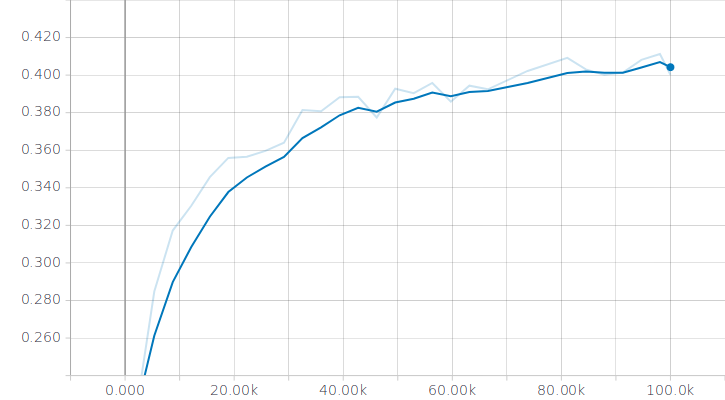
\includegraphics[width=0.45\textwidth]{images/tensorflow/frcnn-map.png}}
        \subfigure[mAP @0.5 IoU]{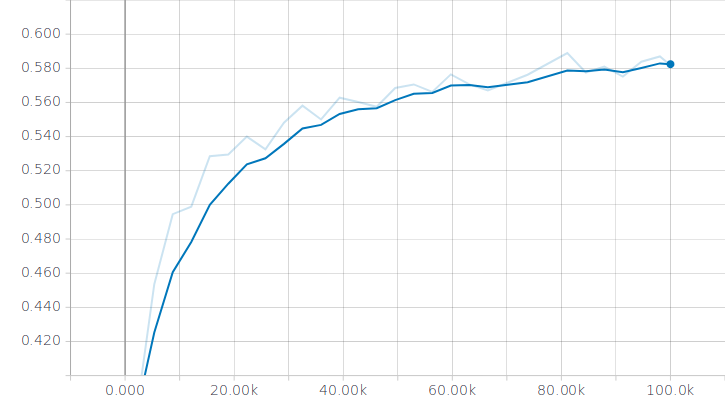
\includegraphics[width=0.45\textwidth]{images/tensorflow/frcnn-map@0-50iou.png}}
        \subfigure[mAP @0.75 IoU]{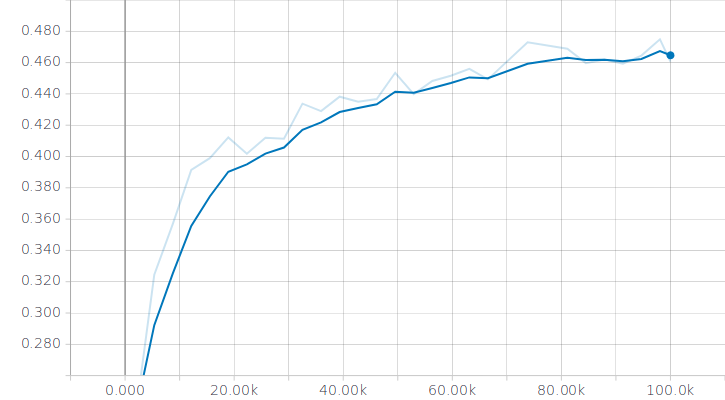
\includegraphics[width=0.45\textwidth]{images/tensorflow/frcnn-map@0-75iou.png}}
    \end{center}
\end{figure}
\newpage \noindent
Even though the mAP is increasing over the duration of the training session it is noticeable that it is not really increasing in performance but
overfiting through the following graphs.
\vspace{0.25cm}
\begin{figure}[hbt!]
    \begin{center}
        \caption{Loss of models}
        \subfigure[Box Classifier Loss]{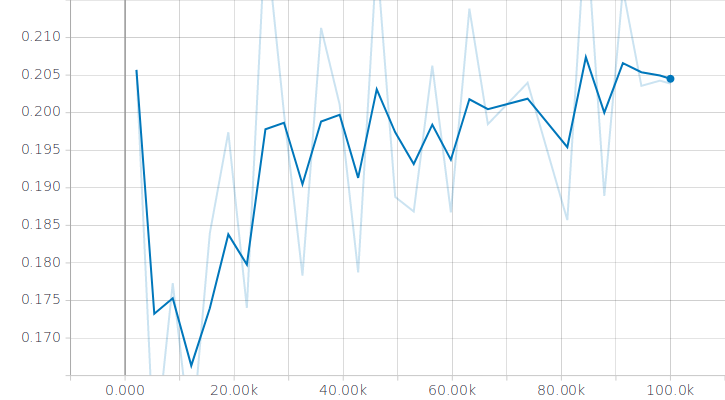
\includegraphics[width=0.45\textwidth]{images/tensorflow/frcnn-classification_loss.png}}
        \subfigure[Box Classifier Localization Loss]{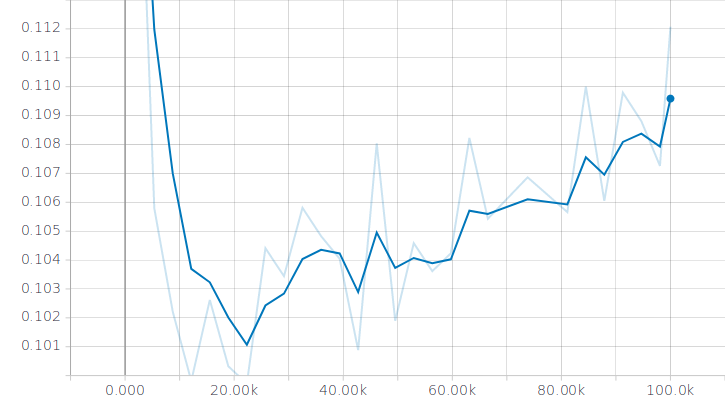
\includegraphics[width=0.45\textwidth]{images/tensorflow/frcnn-box_localization_loss.png}}
        \subfigure[RPN Localization Loss]{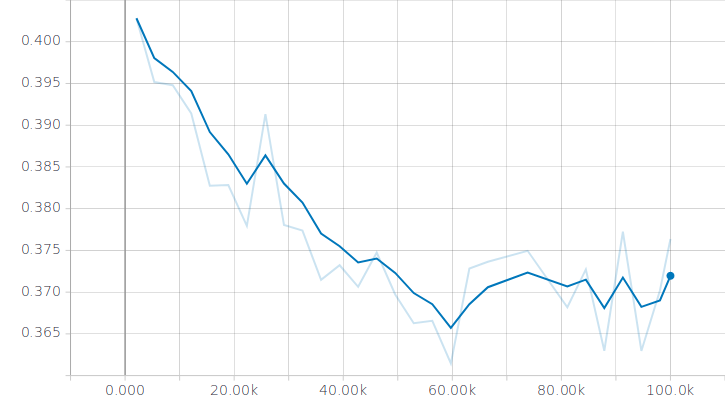
\includegraphics[width=0.45\textwidth]{images/tensorflow/frcnn-rpn_localization_loss.png}}
        \subfigure[RPN Objectness Loss]{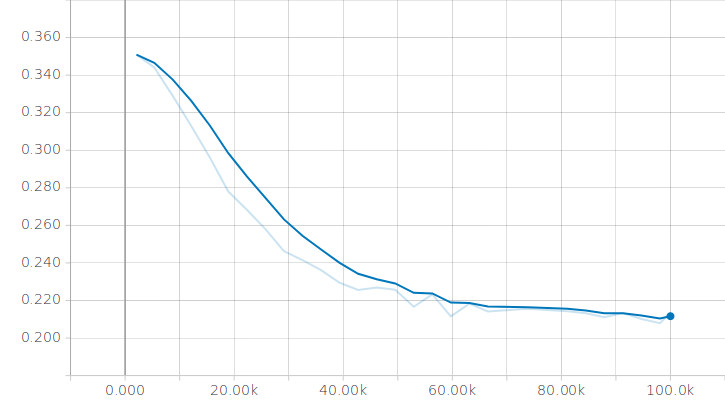
\includegraphics[width=0.45\textwidth]{images/tensorflow/frcnn-rpn_objectness_loss.png}}
        \subfigure[Total Loss]{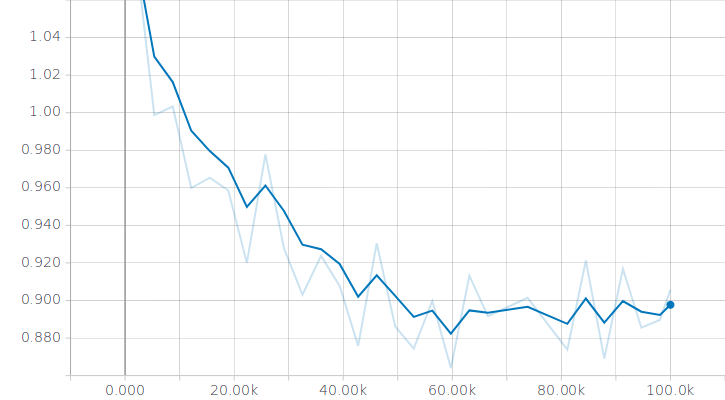
\includegraphics[width=0.45\textwidth]{images/tensorflow/frcnn-total_loss.png}}
    \end{center}
\end{figure}
\end{document}
